In this chapter, we introduce the foundational mathematics required for the study of the Calculus of Variations. The Classical Method leads to the Euler–Lagrange equation, which transforms a variational problem into an ordinary differential equation. Although the Classical Method is not the primary focus of this dissertation, an understanding of this approach provides useful motivation for the development of the Direct Method.

The Direct Method relies on several results from Functional Analysis, alongside an understanding of $L^p$ and Sobolev spaces. Convexity is also an important tool in analysing variational problems and understanding the properties of their solutions. These concepts provide the mathematical framework required to establish the existence of minimisers using the Direct Method. Establishing existence before applying a numerical method is particularly useful, as it allows us to determine whether a variational problem admits a minimiser before attempting to approximate one computationally. Finally we will define and show some examples for the direct method, this will be used in the next chapter on our model problem.

We now formulate the general form of a Calculus of Variations problem. Throughout this dissertation, we focus primarily on minimisation problems. A general model problem can be written in the form
\begin{equation}
\inf \left\{ I(u) = \int_\Omega f(x,u,\nabla u(x)) \, dx : u \in X \right\} = m,
\tag{$\text{P}_\text{General}$}
\label{eq:General_P}
\end{equation}
where the notation follows the formulation given by Dacorogna \cite[p.~3]{dacorogna}.

Here, the various components of the problem are understood as follows:
\begin{itemize}
    \item $\Omega \subset \mathbb{R}^n$, $n \geq 1$, is a bounded open set, with a point in $\Omega$ denoted by $x = (x_1,\dots,x_n)$;

    \item $u : \Omega \rightarrow \mathbb{R}^N$, $N \geq 1$, is the function being minimised, where
    \[
        u = (u^1,\dots,u^N),
    \]
    and
    \[
        \nabla u =
        \left(
        \frac{\partial u^j}{\partial x_i}
        \right)^{1\leq j\leq N}_{1\leq i\leq n}
        \in \mathbb{R}^{N\times n};
    \]

    \item $f : \overline{\Omega} \times \mathbb{R}^N
    \times \mathbb{R}^{N\times n} \rightarrow \mathbb{R}$ is the integrand, assumed to be continuous;

    \item $X$ denotes the space of admissible functions. For example, one may take
    $X = \{u \in C^1(\overline{\Omega}) : u = u_0 \text{ on } \partial\Omega\}$.
\end{itemize}

We are concerned with finding a \textit{minimiser} $\overline{u} \in X$, 
that is, a function satisfying
\[
    I(\overline{u}) \leq I(u), \qquad \forall u \in X.
\]

All the mathematics we develop will be used with the goal of first proving the existence of minimisers and then searching for potential minimisers for these problems. 

\section{The Classical Method}

We begin with a brief overview of the Classical Method, including some examples, in order to establish the ideas that motivate the Direct Method. Following the formulation in Dacorogna \cite[p.~57]{dacorogna}, we consider the one-dimensional variational problem
\begin{equation}
\inf \left\{
I(u): u \in C^1([a,b]),\ u(a)=\alpha,\ u(b)=\beta
\right\},
\tag{B}
\label{eq:Classical_P}
\end{equation}
where $f \in C^2([a,b]\times\mathbb{R}\times\mathbb{R})$ and
\[
    I(u)=\int_a^b f(x,u,u'(x))\,dx.
\]

To motivate the Classical Method, we first recall the analogous minimisation problem in $\mathbb{R}^n$,
\[
\inf\{F(x):x\in X\subset\mathbb{R}^n\}.
\]
For a sufficiently smooth minimiser $\overline{x}$, a necessary condition is
\[
F'(\overline{x})=0.
\]
The second and higher derivatives of $F$ can then be used to investigate the nature of the critical point.

This formulation is a special case of the general variational problem introduced previously. In contrast to the general formulation, the Classical Method considers a one-dimensional domain $[a,b]$ and scalar-valued functions $u:[a,b]\rightarrow\mathbb{R}$. Consequently, the gradient $\nabla u$ is replaced by the ordinary derivative $u'$. The admissible functions are also restricted to $C^1([a,b])$ and are subject to fixed endpoint conditions $u(a)=\alpha$ and $u(b)=\beta$. The endpoint conditions will henceforth be referred to as boundary conditions.

To solve these problems, we can derive the Euler–Lagrange equation that should satisfy any $C^2([a,b])$ minimiser, $\overline{u}$, of $\eqref{eq:Classical_P}$. The Euler–Lagrange equation is analogous to $F'(\overline{x}) = 0$ in $\mathbb{R}^n$. \cite{dacorogna}

The following theorem provides a necessary condition for a sufficiently smooth minimiser of the problem \eqref{eq:Classical_P}. It is stated here in the form used throughout this dissertation; the result corresponds to Theorem 2.1 in Dacorogna \cite[Theorem 2.1, p.~59]{dacorogna}.

\subsection{Euler--Lagrange equation}

\begin{theorem}[Euler--Lagrange equation]
\label{thm:Euler-Lagrange}
    Let $f \in C^2([a,b]\times\mathbb{R}\times\mathbb{R})$, $f = f(x,u,\xi)$, and 
    \begin{equation}
        \inf_{u\in X} \left\{
        I(u) = \int_a^b f(x,u,u'(x))\,dx
        \right\} = m,
    \tag{$\text{P}_\text{Classical}$}
    \label{eq:E-L_P}
    \end{equation}
where
    \[
    X = \{u \in C^1([a,b]) : u(a)=\alpha,\ u(b)=\beta\}.
    \]
\begin{enumerate}

    \item[(i)] If \eqref{eq:E-L_P} admits a minimiser $\overline{u} \in X \cap C^2[(a,b)]$, then, 
    \begin{equation}
        \frac{d}{dx}[f_\xi(x,\overline{u}(x),\overline{u}'(x))] = f_u(x,\overline{u}(x),\overline{u}'(x)).
    \tag{E}
    \label{eq:E-L_E}
    \end{equation}
    
    \item[(ii)] If $\overline{u}$ satisfies \eqref{eq:E-L_E} and if $(u,\xi) \rightarrow f(x,u,\xi)$  is convex for every $x\in[a,b]$, then $\overline{u}$ is a minimiser of \eqref{eq:E-L_P}.

    \item[(iii)] If $(u,\xi) \rightarrow f(x,u,\xi)$  is \textbf{strictly} convex for every $x\in[a,b]$, then the minimiser of \eqref{eq:E-L_P}, if it exists, is unique.
\end{enumerate}

\end{theorem}

\begin{proof}

\begin{enumerate}

    \item[(i)] For every $h \in \mathbb{R}$ and every $v \in C^1[(a,b)]$ with $v(a) = v(b) = 0$ we have
    \[
    I(\overline{u}) \le I(\overline{u} +hv).
    \]
    By setting $\Phi(h) = I(\overline{u} +hv)$, we have that $\Phi \in C^1(\mathbb{R})$ and $\Phi(0) \le \Phi(h)$. We can deduce that $\Phi$ has a relative minimum at $h=0$. Therefore, 
    \[
    \Phi '(0) = \left. \frac{d}{dh}[I(\overline{u} +hv)] \right |_{h=0}=0.
    \]
    Noting that
    \[
    \left. \frac{d\Phi}{dh}\right |_{h=0} = \left. \int_a^b \frac{df}{dh}\right |_{h=0} \, dx,
    \]
    differentiating $f(x,u,u')$ with respect to $h$, where $u=\overline{u} + hv$ and $u'=\overline{u}' + hv'$, gives
    \begin{align*}
        \frac{df}{dh} &= \frac{\partial f}{\partial x} \cancel{\frac{dx}{dh}} + \frac{\partial f}{\partial u}\frac{du}{dh} + \frac{\partial f}{\partial \xi}\frac{du'}{dh}\\
        &= \frac{\partial f}{\partial u}v + \frac{\partial f}{\partial \xi}v',
    \end{align*}
    and hence
    \[
       \Phi'(0) = \int_a^b [f_u(x,\overline{u}(x),\overline{u}'(x))v(x) + f_\xi(x,\overline{u}(x),\overline{u}'(x))v'(x)]\, dx = 0.
    \]
    Using integration by parts on the second term, $f_\xi$, we get
    \begin{align*}
        \int_a^b f_\xi(x,\overline{u}(x),\overline{u}'(x))v'(x)\, dx &= \\
         \left[f_\xi(x,\overline{u}(x),\overline{u}'(x))v(x)\right]_a^b &- \int_a^b \left[ \frac{d}{dx}f_\xi(x,\overline{u}(x),\overline{u}'(x)) \right] v(x) \, dx
    \end{align*}
    Since $v(a) = v(b) = 0$ the first term above vanishes. This leaves us with
    \[
    \Phi'(0) = \int_a^b \left[ f_u(x,\overline{u}(x),\overline{u}'(x)) - \frac{d}{dx}f_\xi(x,\overline{u}(x),\overline{u}'(x)) \right] v(x) \, dx = 0.
    \]
    Applying the fundamental lemma of the calculus of variations, theorem~\ref{thm:Fundamental lemma of the calculus of variations}, described in a further section, we obtain
    \[
        f_u(x,\overline{u}(x),\overline{u}'(x)) - \frac{d}{dx}f_\xi(x,\overline{u}(x),\overline{u}'(x)) = 0
    \]
    which is the Euler-Legrange equation \eqref{eq:E-L_E}.
    \item[(ii)]  See Dacorogna \cite[p.~61]{dacorogna}
    \item[(iii)] See Dacorogna \cite[p.~62]{dacorogna}
\end{enumerate}

\end{proof}

We can and will regularly write the Euler--Lagrange equation in its shorter form
\[
f_y - \frac{d}{dx}f_{\xi} = 0.
\]

Using Theorem~\ref{thm:Euler-Lagrange}, we can obtain minimisers for one-dimensional variational problems. We now consider several examples, starting with the problem of finding the shortest curve joining two points in the plane. Next, Dido's problem before exploring a counterexample that shows the limitation of the Classical Method to be used as motivation for the development of the Direct Method. 

\begin{example}
\label{ex:straight-line}
Find the shortest curve joining the points$A=(x_a,y_a)$ and $B=(x_b,y_b)$ in the plane, where $x_a<x_b$. We begin with the variational functional for arc length given as
\[
J(y)=\int_{x_a}^{x_b}\sqrt{1+(y'(x))^2}\,dx.
\]
The integrand is
\[
f(x,y,\xi)=\sqrt{1+\xi^2},
\]
which is independent of $x$ and $y$. In particular,
$f_y=0$, so the Euler--Lagrange equation \eqref{eq:E-L_E} reduces to
\[
\frac{d}{dx}f_{y'}(x,y(x),y'(x))=0.
\]
Differentiating $f$ with respect to $y'$ gives
\begin{equation}
f_{y'}(x,y(x),y'(x))
=
\frac{y'(x)}{\sqrt{1+(y'(x))^2}}.
\label{eq:fyprime_strightline}
\end{equation}
Hence, by the reduced Euler--Lagrange equation, $f_{y'}$ is constant on $[x_a,x_b]$. Since \eqref{eq:fyprime_strightline}
is a strictly increasing function of $y'$, it follows that $y'$ is constant. Therefore,
\[
y(x)=c_1x+c_2,
\]
for constants $c_1,c_2\in\mathbb{R}$. Thus, the extremal is a straight line, as expected.
\end{example}

\begin{example}[Dido's problem]
\label{ex:Dido's problem}
As discussed previously, Dido's problem concerns finding a curve of prescribed length that encloses the maximum possible area. This problem can be formulated variationally as follows.

Among all sufficiently smooth functions $y$ that are positive on $(0,\ell)$ and satisfy $y(0)=y(\ell)=0$, find a function that minimises
\[
J(y) = -\int_0^{\ell}y(x)\sqrt{1-(y'(x))^2} \, dx.
\]
The integrand is given as 
\[
f(x,y,\xi) = -y\sqrt{1-\xi^2}.
\]

Since $f$ does not explicitly depend on $x$, we can use another reduced form of the Euler--Lagrange equation \eqref{eq:E-L_E}, so that
\begin{equation}
   f-\xi f_\xi = \text{constant}.
   \label{eq:reduced_eulers_dido}
\end{equation}
Substituting our integrand into \eqref{eq:reduced_eulers_dido} gives us
\begin{align*}
 f-y' f_{\xi} &\iff -y\sqrt{1-y'^2} -y' \left(\frac{yy'}{\sqrt{1-y'^2}}\right) = c\\
 &\iff y\sqrt{1-y'^2} + y' \left(\frac{yy'}{\sqrt{1-y'^2}}\right) = \overline{c}\\
 &\iff y(1-y'^2) + yy'^2 = \overline{c}\sqrt{1-y'^2}\\
 &\iff y = \overline{c}\sqrt{1-y'^2}\\
 &\iff \overline{c}y' = \pm\sqrt{\overline{c}^2 - y^2} \quad \text{if $\overline{c} \neq 0$, $y = 0$ otherwise.}
\end{align*}

We now have n ODE to solve. By separation of variables we obtain,
\[
\int \frac{\overline{c}}{\sqrt{\overline{c}^2 - y^2}} \, dy = \pm \int \, dx.
\]
Using the substitution, $y(u) = \overline{c}\sin(u) \implies dy = \overline{c}\cos(u) \,du$, on the left hand side, we get
\[
\int \frac{\overline{c}}{\sqrt{\overline{c}^2 - y^2}} \, dy = \int \frac{\overline{c}^2\cos(u)}{\overline{c}\cos(u)} \, du = \overline{c} u + \tilde{c}.
\]
we therefore obtain 
\[
    x = \overline{c} u + \tilde{c} \implies u = \frac{x}{\overline{c}} + \tilde{c}.
\]
For $\overline{c} \neq 0$ we have 
\[
y(x) = \overline{c} \sin (\frac{x}{\overline{c}} + \tilde{c}).
\]
as a solution to the variation problem and therefore an extremal. Using our boundary conditions we can find a parametric representation as a solution to the problem.
\begin{equation}
    (x(s),y(s)) = \left(-\frac{\ell}{\pi}\cos(\frac{\pi}{\ell}s) - \frac{\ell}{\pi}, \frac{\ell}{\pi}\sin(\frac{\pi}{\ell}s)\right)
    \tag{$*$}
\label{eq:semicircle-param}
\end{equation}the derivation of which is beyond the scope of this example.

\begin{figure}[H]
    \centering
    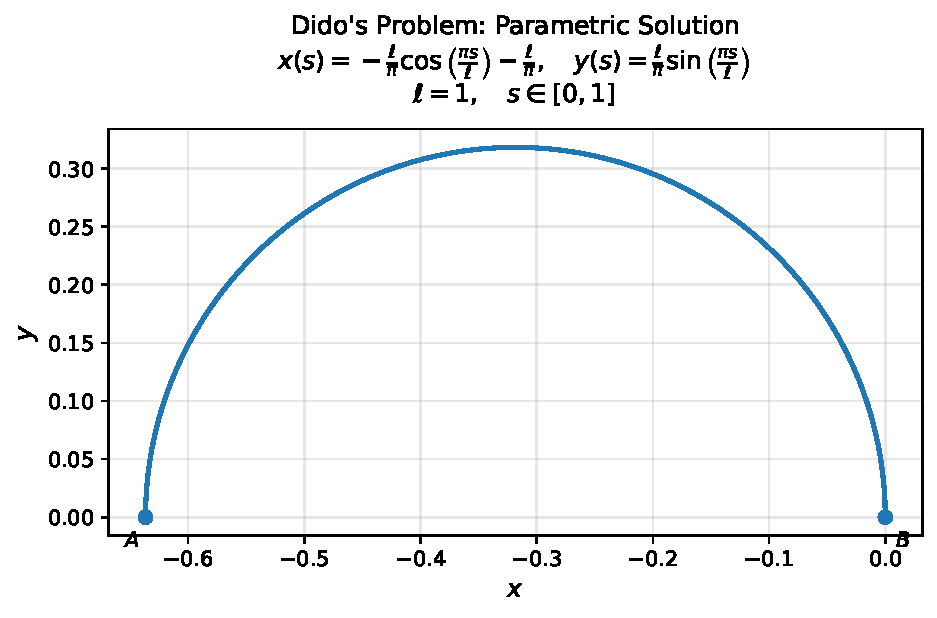
\includegraphics[width=0.7\textwidth]{numerical/outputs/dido.pdf}
    \caption{
        Parametric solution to Dido's problem given in \eqref{eq:semicircle-param} with $\ell = 1, s \in [0,1]$.
        }
    \label{fig:dido-parametric}
\end{figure}

\end{example}

For our counterexample, we consider the Lavrentiev phenomenon and, specifically, the Mani\`a example \cite[p.~70]{dacorogna}. The Euler--Lagrange equation is derived under assumptions on the admissible functions, typically requiring them to be sufficiently smooth ($C^1$ or $C^2$). However, the Mani\`a example demonstrates that a global minimiser of a variational problem need not possess the regularity required by the Classical Method. This motivates the need to consider more general function spaces and provides motivation for the development of the Direct Method.

\begin{example}[Mani\`a Example]
\label{ex:Mania}
Consider the variational problem
\[
J(u)=\int_0^1 (x-u(x)^3)^2(u'(x))^6\,dx,
\]
subject to the boundary conditions 
\[
u(0) = 0, \qquad u(1) = 1.
\] 
The corresponding integrand is
\[
f(x,u,\xi) = (x-u^3)^2\xi^6.
\]
Consider the function $\overline{u}(x) = x^{1/3}$ so that
\[
J(\overline{u}(x)) = \int_0^1 (x - (x^{1/3})^3)^2\left(\frac{1}{3x^{2/3}}\right)^6 = \int_0^1 0 \, dx = 0.  
\]
Since the integrand is non-negative, it follows that for every admissible function $u$
\[
J(u) \geq 0.
\]
Hence $\overline{u}$ is a global minimiser. However the derivative,
\[
\overline{u}'(x)= \frac{1}{3}x^{-2/3},
\]
becomes unbounded as $x \rightarrow 0$. Therefore $\overline{u} \notin C^1([0,1])$. Thus, although $\overline{u}$ is a global minimiser, it does not possess the regularity assumed in the Classical Method. This demonstrates the need to consider broader classes of admissible functions and motivates the development of the Direct Method.
\end{example}


\section{Continuous and H\"older Spaces}

We introduce continuous and H\"older spaces following \cite[Section 1.2, p.~14]{dacorogna}, selecting only those results relevant to this dissertation. Additional remarks and explanations are included where useful for developing the ideas required later.

\subsection{Continuous Functions}

\begin{definition}
    \label{def:Continuous Functions}
    Let $\Omega \subset \mathbb{R}^n$ be an open set.
    \begin{enumerate}
        \item[(ia)] $C^0(\Omega) = C(\Omega)$ is the set of continuous \textbf{functions}, $u : \Omega \rightarrow \mathbb{R}$.
        \item[(ib)] $C^0(\Omega;\mathbb{R}^N) = C(\Omega;\mathbb{R}^N)$ is the set of continuous \textbf{maps}, $u : \Omega \rightarrow \mathbb{R}^N$.
        \item [(ii)] Let $C^0(\overline{\Omega}) = C(\overline{\Omega})$ be the set of continuous functions which can be \textbf{continuously extended} to $\overline{\Omega}$. Similar for maps.
        \item[(iii)] The \textbf{support} of a function $u : \Omega \rightarrow \mathbb{R}$ is defined as 
        \[
            \operatorname{supp} u = \overline{\{x \in \Omega : u(x) \neq 0\}}.
        \]
        \item[(iv)] $C_0(\Omega) = \{u \in C(\Omega) : \operatorname{supp} u \subset \Omega \text{ is compact}\}$.
        \item[(v)] We define the norm over $C(\overline{\Omega})$ by,
        \[
        \|u\|_{C^0} = \sup_{x \in \overline{\Omega}} |u(x)|.
        \]
    \end{enumerate}
\end{definition}

Here are some examples to help build intuition for these definitions.

\begin{example}[Support of a Function]
    \label{ex:Support}

The support of a function is the closure of the region where the function
is \textit{not zero}. Let
\[
u(x) =
\begin{cases}
1-x^2, & \text{if } x\in(-1,1),\\
0, & \text{otherwise}.
\end{cases}
\]

Then:
\begin{itemize}
    \item $u(x)\neq0$ only for $x\in(-1,1)$;

    \item therefore,
    \[
        \{x\in\Omega:u(x)\neq0\}=(-1,1);
    \]

    \item hence, the support is
    \[
        \operatorname{supp}(u)
        =\overline{(-1,1)}
        =[-1,1].
    \]
\end{itemize}

\end{example}

\begin{remark}
    $C(\overline{\Omega})$ equipped with the norm $\|\cdot \|_{C^0}$ is Banach space
\end{remark}

\begin{theorem}[Ascoli--Arzel\`a theorem]
    \label{thm:Ascoli-Arzela}
    Let $\Omega \subset \mathbb{R}^n$ be a bounded domain. Let $K \subset C(\overline{\Omega})$ be bounded such that the following property of equicontinuity holds: $\forall \varepsilon >0$, there exists $\delta > 0$ 
    \[
    |x-y| < \delta \implies |u(x) - u(y)| < \varepsilon, \forall x,y \in \overline{\Omega} \text{ and } \forall u\in K,
    \]
    Then $\overline{K}$ is compact.
\end{theorem}

\begin{example}[Equicontinuity and Ascoli--Arzel\`a]
Consider the sequence of functions on $[0,1]$ given by
\[
    u_n(x)=\frac{x}{n}.
\]
Each $u_n$ is continuous on $[0,1]$, and
\[
    0\leq u_n(x)\leq 1,
\]
for all $x\in[0,1]$ and $n\geq1$. Furthermore, for any
$x_1,x_2\in[0,1]$,
\[
    |u_n(x_1)-u_n(x_2)|
    =\frac{1}{n}|x_1-x_2|
    \leq |x_1-x_2|.
\]
Thus, the family $\{u_n\}$ is equicontinuous, since the same bound
controls the change in every function in the family.

The Ascoli--Arzel\`a theorem (\ref{thm:Ascoli-Arzela}) therefore guarantees that the sequence
contains a uniformly convergent subsequence. In fact, in this example
the whole sequence converges uniformly to the zero function:
\[
    \|u_n\|_{C^0}
    =\sup_{x\in[0,1]}\left|\frac{x}{n}\right|
    =\frac{1}{n}
    \longrightarrow 0.
\]
\end{example}

\begin{remark}
It is important that the hypotheses of the Ascoli--Arzel\`a theorem (\ref{thm:Ascoli-Arzela})  are
satisfied. For example, consider
\[
    u_n(x)=x^n,\qquad x\in[0,1].
\]
Although each $u_n$ is continuous and the sequence is uniformly
bounded, the family $\{u_n\}$ is not equicontinuous on $[0,1]$.
Indeed, the functions become increasingly steep near $x=1$.

Pointwise, we have
\[
    u_n(x)\longrightarrow
    \begin{cases}
        0, & 0\leq x<1,\\
        1, & x=1.
    \end{cases}
\]
whose limit is not continuous. Consequently, the sequence cannot have
a uniformly convergent subsequence.
\end{remark}

\begin{remark}
    We introduce the notation for multi-index derivatives, which may not
    be familiar. Let
    \[
        a=(a_1,\dots,a_n),
    \]
    be a multi-index, where each $a_i$ is a non-negative integer. The
    order of $a$ is defined by
    \[
        |a|=a_1+\cdots+a_n.
    \]
    For a sufficiently differentiable function $u:\Omega\to\mathbb{R}$,
    the derivative corresponding to the multi-index $a$ is
    \[
        D^a u
        =
        \frac{\partial^{|a|}u}
        {\partial x_1^{a_1}\cdots\partial x_n^{a_n}}.
    \]
    In other words, $a_i$ tells us how many times to differentiate with
    respect to $x_i$.
\end{remark}

\begin{definition}
    Let $\Omega \subset \mathbb{R}^n$ be an open set and $k\geq0$ be an integer.
    \begin{enumerate}
        \item[(i)] Set of continuous Functions, $u : \Omega \rightarrow \mathbb{R}$, which have all partial derivatives, $D^a u$, $a \in \mathcal{A}_m$, $0 \leq m \leq k$, is $C^k(\Omega)$.
        \item[(ii)] $C^k(\overline{\Omega})$ is the set of functions whose derivatives up to the order $k$ can be extended continuously to $\overline{\Omega}$. It is equipped with the following norm, 
        \[
        \|u\|_{C^k} = \max_{0\leq|a|\leq k} \sup_{x\in\overline{\Omega}}|D^a u(x)|.
        \]
        \item[(iii)]  $C^k_0(\Omega) = C^k(\Omega)\cap C_0(\Omega)$.

        \item[(iv)]  $C^\infty(\Omega) = \cap_{k=0}^{\infty} C^k(\Omega)$.

        \item[(v)]  $C^\infty_0(\Omega) = C^\infty(\Omega) \cap C_0(\Omega)$.
    \end{enumerate}
\end{definition}

\subsection{H\"older Continuous Functions}

We now turn to the notion of H\"older continuous functions.

\begin{definition}[H\"older Seminorm]
    \label{def:Holder Semi Norm}
    Let $D \subset \mathbb{R}^n$, $u:D\rightarrow\mathbb{R}$ and
    $0<\alpha\leq1$. The H\"older seminorm of $u$ is defined by
    \[
        [u]_{C^{0,\alpha}(D)}
        =
        \sup_{\substack{x,y\in D\\x\neq y}}
        \frac{|u(x)-u(y)|}{|x-y|^\alpha}.
    \]
\end{definition}

\begin{definition}[H\"older Spaces]
    Let $D\subset\mathbb{R}^n$, $u:D\rightarrow\mathbb{R}$ and
    $0<\alpha\leq1$.
    \begin{enumerate}
        \item[(i)] $C^{0,\alpha}(\Omega)$ is the set of functions
        $u\in C(\Omega)$ such that
        \[
            [u]_{C^{0,\alpha}(K)}<\infty
            \qquad
            \text{for every compact set }K\subset\Omega.
        \]
        \item[(ii)] $C^{0,\alpha}(\overline{\Omega})$ is the set of
        functions $u\in C(\overline{\Omega})$ such that
        \[
            [u]_{C^{0,\alpha}(\overline{\Omega})}<\infty.
        \]
        This space is equipped with the norm
        \[
            \|u\|_{C^{0,\alpha}(\overline{\Omega})}
            =
            \|u\|_{C^0(\overline{\Omega})}
            +
            [u]_{C^{0,\alpha}(\overline{\Omega})}.
        \]
        \item[(iii)] For $k\in\mathbb{N}$, let
        \[
            \mathcal{A}_k
            =
            \{a\in\mathbb{N}_0^n:|a|\leq k\}.
        \]
        Then $C^{k,\alpha}(\Omega)$ is the set of functions
        $u\in C^k(\Omega)$ such that
        \[
            [D^a u]_{C^{0,\alpha}(K)}<\infty
            \qquad
            \text{for every compact set }K\subset\Omega
            \text{ and every }a\in\mathcal{A}_k.
        \]
        \item[(iv)] Similarly,
        $C^{k,\alpha}(\overline{\Omega})$ is the set of functions
        $u\in C^k(\overline{\Omega})$ such that
        \[
            [D^a u]_{C^{0,\alpha}(\overline{\Omega})}<\infty
            \qquad
            \text{for every }a\in\mathcal{A}_k.
        \]
        This space is equipped with the norm
        \[
            \|u\|_{C^{k,\alpha}(\overline{\Omega})}
            =
            \|u\|_{C^k(\overline{\Omega})}
            +
            \max_{a\in\mathcal{A}_k}
            [D^a u]_{C^{0,\alpha}(\overline{\Omega})}.
        \]
    \end{enumerate}
\end{definition}

\begin{remark}[Lipschitz Continuity]
    \label{rem:Lipschitz}
    When $\alpha=1$, the space $C^{0,1}(\overline{\Omega})$ is the space
    of \textit{Lipschitz continuous functions}. In particular, a function
    $u\in C(\overline{\Omega})$ is Lipschitz continuous if there exists a
    constant $\gamma>0$ such that
    \[
        |u(x)-u(y)|
        \leq \gamma |x-y|,
        \qquad
        \forall x,y\in\overline{\Omega}.
    \]
    The smallest possible value of $\gamma$ is given by the H\"older
    seminorm
    \[
        \gamma=[u]_{C^{0,1}(\overline{\Omega})}.
    \]
\end{remark}

\begin{example}[H\"older Continuous Function and Computation of the Norm]
    \label{ex:Holder-norm}

    Let $D=[0,1]$ and define
    \[
        u(x)=\sqrt{x}.
    \]
    We compute the H\"older norm of $u$ in
    $C^{0,\frac{1}{2}}([0,1])$.

    First, the $C^0$ norm is
    \[
        \|u\|_{C^0}
        =
        \sup_{x\in[0,1]}|\sqrt{x}|
        =
        1.
    \]
    Next, taking $\alpha=\frac{1}{2}$, the H\"older seminorm is
    \[
        [u]_{C^{0,\frac{1}{2}}}
        =
        \sup_{\substack{x,y\in[0,1]\\x\neq y}}
        \frac{|\sqrt{x}-\sqrt{y}|}{|x-y|^{1/2}}.
    \]
    Using the identity
    \[
        |\sqrt{x}-\sqrt{y}|
        =
        \frac{|x-y|}{\sqrt{x}+\sqrt{y}},
    \]
    we obtain
    \[
        \frac{|\sqrt{x}-\sqrt{y}|}{|x-y|^{1/2}}
        =
        \frac{|x-y|^{1/2}}{\sqrt{x}+\sqrt{y}}.
    \]
    Without loss of generality, suppose that $x>y$. Then
    \[
        \frac{|x-y|^{1/2}}{\sqrt{x}+\sqrt{y}}
        =
        \frac{\sqrt{x-y}}{\sqrt{x}+\sqrt{y}}
        \leq 1.
    \]
    Equality is attained when $y=0$, giving
    \[
        [u]_{C^{0,\frac{1}{2}}}=1.
    \]
    Therefore, the full H\"older norm is
    \[
        \|u\|_{C^{0,\frac{1}{2}}}
        =
        \|u\|_{C^0}
        +
        [u]_{C^{0,\frac{1}{2}}}
        =
        1+1
        =
        2.
    \]

    This example illustrates that $u(x)=\sqrt{x}$ is continuous but not Lipschitz continuous. 
\end{example}

\begin{example}[$C^{1,\alpha}$ Norm in $\mathbb{R}^2$]
    \label{ex:C1alpha-norm}

    Let $\Omega=[0,1]^2$ and define
    \[
        u(x,y)=x^2+y^2.
    \]
    We illustrate the components of the $C^{1,\alpha}(\Omega)$ norm.

    First, we compute the first partial derivatives:
    \[
        u_x=2x,
        \qquad
        u_y=2y.
    \]
    The $C^1$ norm consists of the supremum norms of the function and
    its first derivatives. We have
    \[
        \sup_{\Omega}|u|=2,
        \qquad
        \sup_{\Omega}|u_x|=2,
        \qquad
        \sup_{\Omega}|u_y|=2.
    \]
    Therefore,
    \[
        \|u\|_{C^1}
        =
        \sup_{\Omega}|u|
        +
        \sup_{\Omega}|u_x|
        +
        \sup_{\Omega}|u_y|
        =
        2+2+2=6.
    \]
    Now consider the H\"older seminorms of the first derivatives. For
    $(x,y),(x',y')\in\Omega$,
    \[
        |u_x(x,y)-u_x(x',y')|
        =
        2|x-x'|
        \leq
        2\|(x,y)-(x',y')\|,
    \]
    and similarly,
    \[
        |u_y(x,y)-u_y(x',y')|
        =
        2|y-y'|
        \leq
        2\|(x,y)-(x',y')\|.
    \]
    In particular, when $\alpha=1$, we have
    \[
        [u_x]_{C^{0,1}(\Omega)}
        =
        [u_y]_{C^{0,1}(\Omega)}
        =2.
    \]
    Hence,
    \[
        \max_{|a|=1}[D^a u]_{C^{0,1}(\Omega)}
        =2.
    \]
    Therefore, using the definition of the $C^{1,1}$ norm,
    \[
        \|u\|_{C^{1,1}(\Omega)}
        =
        \|u\|_{C^1(\Omega)}
        +
        \max_{|a|\leq1}[D^a u]_{C^{0,1}(\Omega)}
    \]
    and, with the convention used here,
    \[
        \|u\|_{C^{1,1}(\Omega)}
        =
        6+2=8.
    \]
\end{example}

\section{Lebesgue Spaces}

In this section, we introduce Lebesgue spaces, commonly denoted by $L^p$ spaces. These spaces allow us to work with weaker notions of regularity than those required by the Classical Method, by focusing on the integrability of functions rather than their pointwise smoothness. They are also essential for the definition of Sobolev spaces, which will be introduced in the following section. This provides the language and tools needed to consider whether a function, or its derivatives, are integrable, rather than requiring the stronger pointwise regularity imposed by the Classical Method.

\begin{definition}
    \label{def:L^P Space}
    Let $\Omega \subset \mathbb{R}^n$ be an open set and $1 \le p \le \infty$.  We say that a measurable function $u : \Omega \rightarrow \mathbb{R}$ belongs to $L^p(\Omega)$ if $\|u\|_{L^p}$ is finite. For $p$ finite
    \[
    \|u\|_{L^p} = \left(\int_\Omega |u(x)|^p \, dx\right)^{\frac{1}{p}},
    \]   
    and for $p = \infty$
    \[
    \|u\|_{L^p} = \inf\{\alpha : |u(x)<\alpha \text{ a.e. in } \Omega|\}.
    \]
\end{definition}

\begin{example}[Example of $L^p$ Norms]
    \label{ex:Lp-norm}

    Let $\Omega=(0,1)$ and define
    \[
        u(x)=x.
    \]

    \begin{enumerate}
        \item[(i)] \textbf{Case $p<\infty$.}

        Consider $p=2$. Then
        \[
            \|u\|_{L^2(0,1)}
            =
            \left(\int_0^1 |x|^2\,dx\right)^{1/2}
            =
            \left(\frac{1}{3}\right)^{1/2}
            =
            \frac{1}{\sqrt{3}}.
        \]
        Since the norm is finite, it follows that
        \[
            u\in L^2(0,1).
        \]

        \item[(ii)] \textbf{Case $p=\infty$.}

        The function $u(x)=x$ takes values arbitrarily close to $1$ on
        $(0,1)$, but does not attain the value $1$. Its essential
        supremum is therefore
        \[
            \|u\|_{L^\infty(0,1)}
            =
            \operatorname*{ess\,sup}_{x\in(0,1)}|u(x)|
            =
            1.
        \]
        Since the essential supremum is finite, it follows that
        \[
            u\in L^\infty(0,1).
        \]
    \end{enumerate}
\end{example}

\begin{example}[A Function in $L^1$ but not in $L^2$]
    \label{ex:L1-not-L2}
    Let
    \[
        u(x)=\frac{1}{\sqrt{x}},
    \]
    defined on $\Omega=(0,1)$. First, consider the $L^1$ norm. We have
    \[
        \|u\|_{L^1(0,1)}
        =
        \int_0^1 |u(x)|\,dx
        =
        \int_0^1 x^{-1/2}\,dx
        =
        2.
    \]
    Hence,
    \[
        u\in L^1(0,1).
    \]
    However, for the $L^2$ norm,
    \[
        \|u\|_{L^2(0,1)}^2
        =
        \left(\int_0^1 |u(x)|^2\,dx\right)^\frac{1}2
        =
        \left(\int_0^1 x^{-1}\,dx\right)^\frac{1}2
        =
        \infty.
    \]
    Therefore,
    \[
        u\notin L^2(0,1).
    \]
    This example illustrates that a function may be integrable in the
    $L^1$ sense without being square-integrable. In particular, membership
    of a function in one $L^p$ space does not automatically imply membership
    in another.
\end{example}

\begin{remark}
    \label{rem:conjugate-exponent}

    In the following theorems, we will make use of the \textit{conjugate
    exponent} of $p$, denoted by $p'$. For $1<p<\infty$, it is defined by
    \[
        \frac{1}{p}+\frac{1}{p'}=1,
        \qquad\text{equivalently}\qquad
        p'=\frac{p}{p-1}.
    \]
    For the endpoint cases, if $p=1$, we define $p'=\infty$, while if $p=\infty$, we define $p'=1$.
\end{remark}

\begin{theorem}[Basic properties of $L^p$ spaces]
    \label{thm:Lebesgue-results}

    Let $\Omega\subset\mathbb{R}^n$ be an open set and let
    $1\leq p\leq\infty$. Then the following hold.

    \begin{enumerate}
        \item[(i)] The space $L^p(\Omega)$ is a Banach space. Moreover,
        $L^2(\Omega)$ is a \textbf{Hilbert space} with inner product
        \[
            \langle u,v\rangle
            =
            \int_{\Omega}u(x)v(x)\,dx.
        \]

        \item[(ii)] \textbf{Hölder's inequality:}
        If $u\in L^p(\Omega)$ and $v\in L^{p'}(\Omega)$, where $p'$ is
        the conjugate exponent of $p$, then $uv\in L^1(\Omega)$ and
        \[
            \|uv\|_{L^1(\Omega)}
            \leq
            \|u\|_{L^p(\Omega)}
            \|v\|_{L^{p'}(\Omega)}.
        \]
        In particular, when $p=p'=2$, this gives the
        \textbf{Cauchy--Schwarz inequality}
        \[
            \|uv\|_{L^1(\Omega)}
            \leq
            \|u\|_{L^2(\Omega)}
            \|v\|_{L^2(\Omega)}.
        \]

        \item[(iii)] \textbf{Minkowski's inequality:}
        If $u,v\in L^p(\Omega)$, then
        \[
            \|u+v\|_{L^p(\Omega)}
            \leq
            \|u\|_{L^p(\Omega)}
            +
            \|v\|_{L^p(\Omega)}.
        \]

        \item[(iv)] \textbf{Riesz theorem:}
        If $1\leq p<\infty$ and $\varphi\in(L^p(\Omega))'$, then,
        under the appropriate assumptions, there exists
        $u\in L^{p'}(\Omega)$ such that
        \[
            \langle\varphi,f\rangle
            =
            \varphi(f)
            =
            \int_{\Omega}u(x)f(x)\,dx,
            \qquad
            \forall f\in L^p(\Omega).
        \]
        and moreover 
        \[
            \|u\|_{L^{p'}} = \|\varphi\|_{{(L^p)}'}.
        \]
        \item[(v)] The space $L^p(\Omega)$ is separable for
        $1\leq p<\infty$ and reflexive for $1<p<\infty$.

        \item[(vi)] If $1\leq p<\infty$ and $u\in L^p(\Omega)$, then there
        exists a sequence $(u_\nu)\subset C^\infty_0(\Omega)$ such that
        \[
            \lim_{\nu\rightarrow\infty}
            \|u_\nu-u\|_{L^p(\Omega)}
            =
            0.
        \]
        This result is false in general for $p=\infty$.
    \end{enumerate}
\end{theorem}

\begin{remark}[Duality of $L^p$ Spaces]
    \label{rem:Lp-duality}

    To summarise the duality results, we have
    \[
        (L^p(\Omega))' \cong L^{p'}(\Omega),
        \qquad 1<p<\infty,
    \]
    where $p'$ is the conjugate exponent of $p$. In particular,
    \[
        (L^2(\Omega))' \cong L^2(\Omega),
    \]
    since $2'=2$. At the endpoint $p=1$, we have
    \[
        (L^1(\Omega))' \cong L^\infty(\Omega).
    \]
    However, the corresponding result does not hold for $p=\infty$.
    In general,
    \[
        L^1(\Omega)\subsetneq (L^\infty(\Omega))'.
    \]
\end{remark}

We will now consider convergence in $L^p$ spaces. The natural notion of \textit{strong convergence} is induced by the $L^p$ norm. We will also introduce the notion of \textit{weak convergence}, which will be important when considering the Direct Method.

\begin{definition}[Convergence in $L^p$ spaces]
    \label{def:Lp-convergence}

    Let $\Omega\subset\mathbb{R}^n$ be an open set and let
    $1\leq p\leq\infty$.

    \begin{enumerate}
        \item[(i)] A sequence $(u_\nu)$ is said to \textbf{strongly converge}
        to $u$ in $L^p(\Omega)$ if $u_\nu,u\in L^p(\Omega)$ and
        \[
            \lim_{\nu\rightarrow\infty}
            \|u_\nu-u\|_{L^p(\Omega)}
            =0.
        \]
        We denote this by
        \[
            u_\nu\rightarrow u
            \qquad\text{in }L^p(\Omega).
        \]

        \item[(ii)] If $1\leq p<\infty$, a sequence $(u_\nu)$ is said to
        \textbf{weakly converge} to $u$ in $L^p(\Omega)$ if
        $u_\nu,u\in L^p(\Omega)$ and
        \[
            \lim_{\nu\rightarrow\infty}
            \int_\Omega
            [u_\nu(x)-u(x)]\varphi(x)\,\mathrm{d}x
            =0,
            \qquad
            \forall\varphi\in L^{p'}(\Omega).
        \]
        We denote this by
        \[
            u_\nu\rightharpoonup u
            \qquad\text{in }L^p(\Omega).
        \]

        \item[(iii)] If $p=\infty$, a sequence $(u_\nu)$ is said to
        \textbf{weak-$*$ converge} to $u$ in $L^\infty(\Omega)$ if
        $u_\nu,u\in L^\infty(\Omega)$ and
        \[
            \lim_{\nu\rightarrow\infty}
            \int_\Omega
            [u_\nu(x)-u(x)]\varphi(x)\,\mathrm{d}x
            =0,
            \qquad
            \forall\varphi\in L^1(\Omega).
        \]
        We denote this by
        \[
            u_\nu\rightharpoonup^* u
            \qquad\text{in }L^\infty(\Omega).
        \]
    \end{enumerate}
\end{definition}


\begin{example}[Weak Convergence in $L^p$]
    \label{ex:weak-convergence}

    Let $\Omega=(0,1)$ and define
    \[
        u_\nu(x)=\sin(2\pi \nu x).
    \]
    We claim that
    \[
        u_\nu\rightharpoonup 0
        \qquad\text{in }L^p(0,1),
        \qquad 1<p<\infty.
    \]
    Indeed, let $\varphi\in L^{p'}(0,1)$. Then
    \[
        \int_0^1
        u_\nu(x)\varphi(x)\,\mathrm{d}x
        =
        \int_0^1
        \sin(2\pi \nu x)\varphi(x)\,\mathrm{d}x
        \longrightarrow 0
        \qquad\text{as }\nu\rightarrow\infty.
    \]
    This follows from the oscillatory nature of $\sin(2\pi\nu x)$
    and the Riemann--Lebesgue lemma. Therefore,
    \[
        u_\nu\rightharpoonup0
        \qquad\text{in }L^p(0,1).
    \]
    However, the convergence is not strong. For example, when $p=2$,
    \[
        \|u_\nu\|_{L^2(0,1)}^2
        =
        \int_0^1\sin^2(2\pi\nu x)\,\mathrm{d}x
        =
        \frac12,
    \]
    and hence
    \[
        \|u_\nu\|_{L^2(0,1)}
        =
        \frac{1}{\sqrt{2}}
        \not\longrightarrow0.
    \]
    
    Thus, weak convergence does not in general imply strong convergence.
\end{example}

\begin{example}[Weak-$*$ Convergence in $L^\infty$]
    \label{ex:weak-star-convergence}

    Let $\Omega=(0,1)$ and define the sequence $(u_\nu)$ by
    \[
        u_\nu(x)
        =
        (-1)^k,
        \qquad
        x\in
        \left[\frac{k}{\nu},\frac{k+1}{\nu}\right),
        \quad
        k=0,\ldots,\nu-1.
    \]
    Thus, $u_\nu$ alternates between $1$ and $-1$ on increasingly
    fine subintervals of $(0,1)$. In particular,
    \[
        \|u_\nu\|_{L^\infty(0,1)}=1,
    \]
    so the sequence is bounded in $L^\infty(0,1)$.

    For every $\varphi\in L^1(0,1)$, the increasingly rapid oscillations
    of $u_\nu$ imply
    \[
        \int_0^1 u_\nu(x)\varphi(x)\,\mathrm{d}x
        \longrightarrow 0
        \qquad\text{as }\nu\rightarrow\infty.
    \]
    Hence,
    \[
        u_\nu\rightharpoonup^*0
        \qquad\text{in }L^\infty(0,1).
    \]
    However,
    \[
        \|u_\nu-0\|_{L^\infty(0,1)}
        =
        1
    \]
    for every $\nu$. Therefore, $u_\nu$ does not converge strongly to
    zero in $L^\infty(0,1)$.

    This example illustrates that weak-$*$ convergence does not in
    general imply strong convergence in $L^\infty$.
\end{example}

\begin{definition}
    $u \in L^p_{loc}(\Omega)$ if $u \in L^p(\Omega')$ for every open set $\Omega'$ compactly contained in $\Omega$
\end{definition}
\begin{theorem}[Fundamental lemma of the calculus of variations]
\label{thm:Fundamental lemma of the calculus of variations}
Let $\Omega$ be an open set of $\mathbb{R}^n$ and $u \in L^1_{loc}(\Omega)$ be such that 
$$
\int_\Omega u(x)\, \varphi(x) \, \mathrm{d}x = 0, \qquad \forall \varphi \in C^{\infty}_0(\Omega)
$$
then $u = 0$, a.e. in $\Omega$.
\end{theorem}
\begin{proof}
Following the method presented by Dacorogna~\cite[p.~27]{dacorogna}, we first prove the theorem under the stronger assumption that \(u\in L^2(\Omega)\). Recall that \(L^2(\Omega)\subset L^1_{\mathrm{loc}}(\Omega)\). Let \(\epsilon>0\). By part~(iv) of the Riesz theorem, stated in Theorem~\ref{thm:Lebesgue-results}, and since \(u\in L^2(\Omega)\), there exists \(\varphi\in C_0^\infty(\Omega)\) such that
\[
    \|u-\varphi\|_{L^2}\leq\epsilon.
\]
By the hypothesis of the fundamental lemma,
\[
    \int_\Omega u\varphi\,dx=0.
\]
Therefore,
\[
\begin{aligned}
    \|u\|_{L^2}^2
    &=\int_\Omega u^2\,dx\\
    &=\int_\Omega u^2\,dx-\int_\Omega u\varphi\,dx\\
    &=\int_\Omega u(u-\varphi)\,dx.
\end{aligned}
\]
Applying Hölder's inequality, given in part~(ii) of Theorem~\ref{thm:Lebesgue-results}, we obtain
\[
    \|u\|_{L^2}^2
    \leq
    \|u\|_{L^2}\|u-\varphi\|_{L^2}
    \leq
    \epsilon\|u\|_{L^2}.
\]
Since \(\epsilon>0\) is arbitrary, it follows that
\[
    \|u\|_{L^2}=0.
\]
Hence \(u=0\) almost everywhere in \(\Omega\), as required.
\end{proof}

\section{Sobolev Spaces}
\label{sec:Sobolev_Spaces}
In this section, we introduce Sobolev spaces, commonly denoted by \(W^{k,p}(\Omega)\), where \(1\leq p\leq\infty\) and \(k\in\mathbb{N}\). We weaken the notion of differentiation so that we can work with functions that are not necessarily classically differentiable, while retaining the ability to integrate by parts. This is particularly useful in the Direct Method, where we need to control both a function and its derivatives. We begin by introducing weak derivatives before defining Sobolev spaces and giving some examples for intuition. For further reading, see Dacorogna~\cite[p.~30]{dacorogna}.

\subsubsection{Weak Partial Derivative}
\begin{definition}
    Let $\Omega \subset \mathbb{R}^N$ be open and $u\in L^1_{loc}(\Omega)$. We say that:
    \begin{enumerate}
        \item[(i)]
            $v\in L^1_{loc}(\Omega)$ is the \textit{weak partial derivative} of $u$ with respect to $x_i$ if
            \[
            \int_\Omega v(x)\,\varphi(x)\, dx = - \int_\Omega \, u(x) \frac{\partial\varphi}{\partial x_i} \, dx, \quad \forall \varphi \in C^\infty_0(\Omega).
            \]
            by abuse of notation, $v = \delta u / \delta x_i$ or $u_{x_i}$.
        \item[(ii)]
            We say that $u$ is \textit{weakly differentiable} if the weak partial derivatives, $u_{x_i}, \dots , u_{u_n}$, exist.
    \end{enumerate}
\end{definition}

\begin{example}[Weak derivative example]
\label{ex:Weak derivative example}
    Let us consider the function
    \[
        u(x)=|x|, \qquad x\in(-1,1).
    \]
    This function is not classically differentiable at \(x=0\). However, we can show that it possesses a weak derivative. Define
    \[
        v(x)=
        \begin{cases}
            -1, & x<0,\\
            1, & x>0,
        \end{cases}
    \]
    or, equivalently,
    \[
        v(x)=\operatorname{sgn}(x).
    \]
    We want to show that \(v\) is the weak derivative of \(u\). From the definition of a weak derivative, we require
    \[
        \int_{-1}^1 v(x)\varphi(x)\,dx
        =
        -\int_{-1}^1 |x|\varphi'(x)\,dx,
        \qquad
        \forall \varphi\in C_0^\infty(-1,1).
    \]
    Splitting the integral at \(x=0\) gives
   \[
    -\int_{-1}^1 |x|\varphi'(x)\,dx = \int_{-1}^0 x\varphi'(x)\,dx -\int_{0}^1 x\varphi'(x)\,dx.
    \]
    Integrating by parts,
    \[
    \int_{-1}^0 x\varphi'(x)\,dx = [x\varphi(x)]_{-1}^0 - \int_{-1}^0 \varphi(x)\,dx = -\int_{-1}^0 \varphi(x) \,dx,
    \]
    where the boundary terms vanish since
    \(\varphi\in C_0^\infty(-1,1)\). Similarly,
    \[
        -\int_0^1 x\varphi'(x)\,dx
        =
        \int_0^1 \varphi(x)\,dx.
    \]
    Hence,
    \[
    -\int_{-1}^1 |x|\varphi'(x)\,dx = -\int_{-1}^0 \varphi(x)\,dx  + \int_{0}^1 \varphi(x)\,dx = \int_{-1}^1 \operatorname{sgn}(x)\varphi(x)\,dx.
    \]
    Therefore,
    \[
        u_x=\operatorname{sgn}(x)
    \]
    is the weak derivative of \(u\).
\end{example}

We will now consider Sobolev spaces with weak derivatives of order one, denoted by $W^{1,p}(\Omega)$.

\subsection{Sobolev Norms}
\begin{definition}
    \label{def: Sobolev k =1}
    Let $\Omega \subset \mathbb{R}^n$ be an open set and $1 \le p \le \infty$.
    \begin{enumerate}
        \item[(i)]  We let $W^{1,p}(\Omega)$ be the set of functions $u : \Omega \rightarrow \mathbb{R}^n$, $u \in L^P(\Omega)$, whose weak partial derivatives $u_{x_i} \in L^p(\Omega)$ for every $i=1,...,n$. This space has the following norm,
        \[
        \|u\|_{W^{1,p}(\Omega)}
        =
        \begin{cases}
        \left(
        \|u\|_{L^p(\Omega)}^p
        +
        \|\nabla u\|_{L^p(\Omega)}^p
        \right)^{1/p},
        & 1\leq p<\infty, \\[1.5ex]
        \max\left\{
        \|u\|_{L^\infty(\Omega)},
        \|\nabla u\|_{L^\infty(\Omega)}
        \right\},
        & p=\infty.
        \end{cases}
        \]
        In the special case of \(p=2\), the space \(W^{1,2}(\Omega)\) is commonly denoted by \(H^1(\Omega)\), as it forms a Hilbert space with its natural inner product;
        
        \item[(ii)] For $1\leq p<\infty$, the set $W_0^{1,p}(\Omega)$ is the closure of $C_0^\infty(\Omega)$ functions in $W^{1,p}(\Omega)$. If $\Omega$ is bounded then $u \in W_0^{1,p}(\Omega)$ is such that $u \in W^{1,p}(\Omega)$ and $u=0$ on $\delta\Omega$;

        \item[(iii)] $u \in u_0 + W^{1,p}_0(\Omega)$ means $u,u_0 \in W^{1,p}(\Omega)$ and $u-u_0 \in W^{1,p}_0(\Omega)$;

        \item[(iv)] We let $W^{1,\infty}_0 = W^{1,\infty} \cap W^{1,1}_0$.
    \end{enumerate}
\end{definition}

\begin{example}[Computing the Sobolev norm]
\label{ex:Sobolev Norm example}
    Let us again consider the function
    \[
        u(x)=|x|, \qquad x\in(-1,1).
    \]
    From Example \ref{ex:Weak derivative example}, we have
    \[
        u_x=\operatorname{sgn}(x).
    \]

    For \(p=1\), from part (i) of Definition \ref{def: Sobolev k =1},
    \[
        \|u\|_{W^{1,1}}
        =
        \|u\|_{L^1}+\|u_x\|_{L^1}.
    \]
    We compute each term separately:
    \[
        \|u\|_{L^1}
        =
        \int_{-1}^1 |x|\,dx
        =
        2\int_0^1 x\,dx
        =
        1,
    \]
    and
    \[
        \|u_x\|_{L^1}
        =
        \int_{-1}^1 |\operatorname{sgn}(x)|\,dx
        =
        \int_{-1}^1 1\,dx
        =
        2.
    \]
    Therefore,
    \[
        \|u\|_{W^{1,1}}=3.
    \]

    For \(p=2\),
    \[
        \|u\|_{W^{1,2}}
        =
        \left(
        \|u\|_{L^2}^2+\|u_x\|_{L^2}^2
        \right)^{1/2}.
    \]
    We have
    \[
        \|u\|_{L^2}^2
        =
        \int_{-1}^1 |x|^2\,dx
        =
        \frac{2}{3},
    \]
    and
    \[
        \|u_x\|_{L^2}^2
        =
        \int_{-1}^1 |\operatorname{sgn}(x)|^2\,dx
        =
        \int_{-1}^1 1\,dx
        =
        2.
    \]
    Hence,
    \[
        \|u\|_{W^{1,2}}
        =
        \sqrt{\frac{2}{3}+2}
        =
        \sqrt{\frac{8}{3}}.
    \]
    
    Finally, for \(p=\infty\),
    \[
        \|u\|_{W^{1,\infty}}
        =
        \max\left\{
            \|u\|_{L^\infty},
            \|u_x\|_{L^\infty}
        \right\}.
    \]
    Since
    \[
        \|u\|_{L^\infty}
        =
        \operatorname*{sup}_{x\in(-1,1)} |x|
        =
        1,
    \]
    and
    \[
        \|u_x\|_{L^\infty}
        =
        \operatorname*{sup}_{x\in(-1,1)}
        |\operatorname{sgn}(x)|
        =
        1,
    \]
    we obtain
    \[
        \|u\|_{W^{1,\infty}}=1.
    \]
\end{example}

We now consider Sobolev spaces for $k \neq 1$. 

\begin{definition}
    \label{def: Sobolev general k}
    Let $\Omega \subset \mathbb{R}^n$ be an open set and $1 \le p \le \infty$.\
\begin{enumerate}
    \item[(i)] For higher-order derivatives, we define the Sobolev spaces as follows. 
    For $k\in\mathbb{N}$, $k\geq1$, the space $W^{k,p}(\Omega)$ consists of all functions
    $u\in L^p(\Omega)$ whose weak partial derivatives $D^\alpha u$ belong to
    $L^p(\Omega)$ for every multi-index $\alpha$ satisfying $0\leq|\alpha|\leq k$.
    The corresponding norm is defined by
    \[
    \|u\|_{W^{k,p}(\Omega)}
    =
    \begin{cases}
    \displaystyle
    \left(
    \sum_{|\alpha|\leq k}
    \|D^\alpha u\|_{L^p(\Omega)}^p
    \right)^{1/p},
    & 1\leq p<\infty, \\[3ex]
    \displaystyle
    \max_{|\alpha|\leq k}
    \|D^\alpha u\|_{L^\infty(\Omega)},
    & p=\infty;
    \end{cases}
    \]
    
    \item[(ii)] If $1\leq p<\infty$, the set $W_0^{k,p}(\Omega)$ is the closure of $C_0^\infty(\Omega)$ in $W^{k,p}(\Omega)$ and $W_0^{k,p}(\Omega)= W^{k,\infty}(\Omega) \cap W_0^{k.1}(\Omega)$.
\end{enumerate}

\end{definition}

Having defined $W^{1,p}(\Omega)$, we can interpret $k$ as the largest order of weak derivative controlled by the space. Thus, increasing $k$ requires progressively higher-order regularity:

\begin{enumerate}
\item $k=0$: control of the function itself through integrability;
\item $k=1$: control of first-order weak derivatives;
\item $k=2$: control of second-order weak derivatives;
\item higher $k$: control of higher-order weak derivatives.
\end{enumerate}

$p$, on the other hand, determines the integrability of the function and its derivatives. Roughly speaking, it determines how strongly large values are penalised in the corresponding $L^p$ norm. Smaller values of $p$ allow greater variation, while larger values place greater emphasis on large values. In the case of $p=\infty$, the $L^\infty$ norm essentially measures the  maximum value.

Therefore, $k$ determines \textit{what order of derivative} is controlled, while $p$ determines \textit{how the size of those derivatives is measured}.

\begin{example}[Sobolev norm for general $k$]
    \label{ex:Sobolev general k}
    Let us consider the function
    \[
        u(x)=x^2, \qquad x\in(-1,1).
    \]
    We compute the $W^{2,2}$ norm for this function. We have
    \[
        \|u\|^2_{W^{2,2}}
        =
        \|u\|^2_{L^2}
        +
        \|u'\|^2_{L^2}
        +
        \|u''\|^2_{L^2}.
    \]
    Our derivatives are
    \[
        u(x)=x^2, \qquad u'(x)=2x, \qquad u''(x)=2.
    \]
    Using the definition of the $L^2$ norm, we have
    \[
        \|u\|_{L^2}^2
        =
        \int_{-1}^1 x^4\,dx
        =
        \frac{2}{5},
    \]
    \[
        \|u'\|_{L^2}^2
        =
        \int_{-1}^1 (2x)^2\,dx
        =
        \int_{-1}^1 4x^2\,dx
        =
        \frac{8}{3},
    \]
    and
    \[
        \|u''\|_{L^2}^2
        =
        \int_{-1}^1 4\,dx
        =
        8.
    \]
    Therefore,
    \[
        \|u\|_{W^{2,2}}^2
        =
        \frac{2}{5}
        +
        \frac{8}{3}
        +
        8
        =
        \frac{166}{15}.
    \]
    Hence,
    \[
        \|u\|_{W^{2,2}}
        =
        \sqrt{\frac{166}{15}}.
    \]
\end{example}

\begin{example}[A function not belonging to $W^{k,p}$ for $k>1$]
\label{ex:Absolute value not Wkp}
We again consider the function
    \[  
    u(x)=|x|, \qquad x\in(-1,1).
    \]
From Example \ref{ex:Weak derivative example}, we know that its weak first derivative is
\[
    u'(x)=\operatorname{sgn}(x).
\]
Since both $u$ and $u'$ belong to $L^p(-1,1)$ for any
$1\leq p\leq\infty$, it follows that
\[  
u\in W^{1,p}(-1,1).
\]

However, to belong to $W^{2,p}(-1,1)$, the function must also allow a second weak derivative belonging to $L^p(-1,1)$. As demonstrated in Example 1.29 of Dacorogna~\cite[p.~30]{dacorogna}, differentiating $u'$ gives
\[
u''=2\delta_0,
\]
where $\delta_0$ denotes the Dirac mass. The Dirac mass is not an $L^p$ therefore,
\[
    u\notin W^{2,p}(-1,1).
\]
we conclude that
\[
    u\notin W^{k,p}(-1,1)
    \quad\text{for all } k>1.
\]
This example shows that increasing $k$ asks for stronger regularity on a function. Even though $u(x)=|x|$ has a weak first derivative and belongs to $W^{1,p}(-1,1)$, it does not allow a second weak derivative in $L^p(-1,1)$ and so it cannot belong to any $W^{k,p}(-1,1)$ with $k>1$.
\end{example}

\subsection{Poincar\'e Inequality}

\begin{theorem}
    \label{thm:Poincare Inequality}
    Let $\Omega \subset \mathbb{R}^n$ be a bounded open set and $1\leq p \leq \infty$. Then there exists $\gamma = \gamma(\Omega,p) > 0$  so that, 
    $$
        \|u\|_{L^p \text{ or } W^{1,p}} \le \gamma\|\nabla u\|_{L^p}
        \, \quad \forall u \in W^{1,p}_0.
    $$
\end{theorem}
For a proof, see Dacorogna~\cite[p.~45]{dacorogna}.

\section{Convex Analysis}

Convex analysis is a broad area of mathematics, so this section focuses only on the concepts relevant to the Direct Method. We introduce the definition of convex set, convex functions, and some conditions, alongside examples to illustrate these ideas.

\subsection{Convex Sets}

\begin{definition}
    The set $\Omega \subset \mathbb{R}^n$ is said to be convex if from for every $x,y \in \Omega$ and every $\lambda \in [0,1]$ we have $\lambda x + (1-\lambda)y \in \Omega$.
\end{definition}

\begin{example}[Convex Set Example]

 Let
 $$
 \Omega=(0,1).
 $$
 Choose
 $$
 x=0.2,\qquad y=0.8,\qquad \lambda=0.25.
 $$
 Then
 $$
 \lambda x + (1-\lambda)y
 =
 0.25(0.2)+0.75(0.8)
 =
 0.65.
 $$
 Since $0.65 \in (0,1)$, the point remains in the set.

 In fact, every weighted average of two points in $(0,1)$ remains in $(0,1)$. Therefore $(0,1)$ is convex.
\end{example}

\subsection{Convex Functions}

\begin{definition}
    Let $\Omega \subset \mathbb{R}^n$ be convex. The Function $f : \Omega \rightarrow \mathbb{R}$ is said to be convex if for every $x,y\in \Omega$ and every $\lambda \in [0,1]$, the following inequality holds

$$
f(x) \ge f(y) + \langle \nabla f(y);x-y\rangle, \forall x,y \in \mathbb{R}^n
$$
\end{definition}

\begin{example}
Let $\Omega = \mathbb{R}^n$ and define
$$
    f(x) = |x|^2.
$$
Then
$$
    \nabla f(x)=2x.
$$
To verify that $f$ is convex, take $x,y\in\mathbb{R}^n$. The convexity condition for a differentiable function is
$$
    f(x)\geq f(y)+\langle \nabla f(y),x-y\rangle.
$$
Substituting $f(x)=|x|^2$ and $\nabla f(y)=2y$ gives
$$
    |x|^2\geq |y|^2+2\langle y,x-y\rangle.
$$
Rearranging,
$$
    |x|^2-|y|^2-2\langle y,x-y\rangle
    =|x-y|^2\geq0.
$$
Hence the convexity inequality holds, and therefore
$$
    f(x)=|x|^2
$$
is convex. 

We can also verify this visually, as illustrated in Figure~\ref{fig:convex_function}, it can be observed that the function $f(x)=|x|^2$ is convex.

\begin{figure}[H]
    \centering
    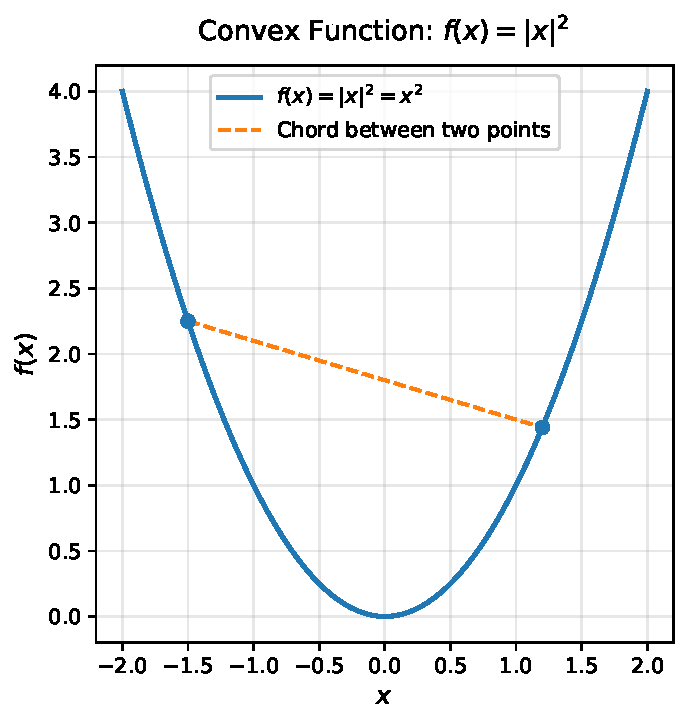
\includegraphics[width=0.6\textwidth]{numerical/outputs/convex_function.pdf}
    \caption{
        The function $f(x)=|x|^2$, with a chord illustrating its convexity.
    }
    \label{fig:convex_function}
\end{figure}

\end{example}

\subsection{Convexity Conditions}

\begin{theorem}
    Let $f:\mathbb{R}^n \rightarrow \mathbb{R}$ and $f \in C^1(\mathbb{R})$. We denote the scalar product in $\mathbb{R}^n$ by $\langle.;.\rangle$. The following assertions are equivalent.
    \begin{enumerate}
        \item[(i)] the function $f$ is \emph{convex};
        \item[(ii)] for every $x,y\in\mathbb{R}^n$, the following inequality holds
        \[
        f(x) \ge f(y) + \langle \nabla f(y);x-y\rangle;
        \]
        \item[(iii)] for every $x,y\in\mathbb{R}^n$, the following inequality is vails
        \[
        \langle \nabla f(x) - \nabla f(y);x-y\rangle \geq 0;
        \]
        \item[(iv)] If $f\in C^2(\mathbb{R}^n)$, then for every $x,v\in\mathbb{R}^n$,
        \[
            \langle \nabla^2 f(x)v,v\rangle \geq 0.
        \]
        This is equivalent to saying that the Hessian matrix $\nabla^2 f(x)$ is positive semidefinite.
    \end{enumerate}
\end{theorem}

\section{The Direct Method}

In this section, we develop the Direct Method of the Calculus of Variations. The Direct Method provides a framework for proving the existence of minimisers for a given functional and the conditions under which minimisers exist. We start by extending the model problem, (\ref{eq:Classical_P}), introduced at the beginning of the chapter, building on the theory of Sobolev spaces developed in Section \ref{sec:Sobolev_Spaces}. We then consider model problems to develop an intuition for the method. Following this, we introduce the main existence results and derive the Euler--Lagrange equation for the Direct Method in the setting of $\overline{u} \in W^{1,p}$. As with the previous sections, we will primarily follow Dacorogna \cite{dacorogna}, particularly Chapter 3, while also drawing on examples and notation from Rindler \cite{rindler}.


For the Direct Method, we consider the problem
\[
\tag{$\text{P}_\text{direct}$}
\inf \left\{ I(u) = \int_\Omega f(x,u(x),\nabla u(x))\,dx
: u\in u_0+W_0^{1,p}(\Omega) \right\}=m,
\label{eq:Direct_P}
\]
where
\begin{itemize}
\item $\Omega\subset\mathbb{R}^n$ is a bounded open set;
\item $f:\overline{\Omega}\times\mathbb{R}\times\mathbb{R}^n\rightarrow\mathbb{R}$, with $f=f(x,u,\xi)$;
\item $u \in u_0\in W^{1,p}_0(\Omega)$ means that $u,u_0\in W_0^{1,p}(\Omega)$ and $u-u_0\in W_0^{1,p}(\Omega)$. (this corresponds to $u=u_0$ on $\partial\Omega$.)
\end{itemize}
We will show that, under suitable hypotheses, the problem, \ref{eq:Direct_P}, admits a solution $\overline{u}\in u_0+W_0^{1,p}(\Omega)$. In particular, we will require the following two main hypotheses:
\begin{enumerate}
\item \textit{Convexity:} for every $(x,u)\in\overline{\Omega}\times\mathbb{R}$, the function
\(    \xi\mapsto f(x,u,\xi)
   \)
is convex.
\item \textit{Coercivity:} there exist $p>q\geq1$ and constants $\alpha_1>0$, $\alpha_2,\alpha_3\in\mathbb{R}$ such that
\[
f(x,u,\xi)
\geq
\alpha_1|\xi|^p+\alpha_2|u|^q+\alpha_3,
\]
for all $(x,u,\xi)\in\overline{\Omega}\times\mathbb{R}\times\mathbb{R}^n$.
\end{enumerate}


The \textit{Dirichlet integral} which has integrand
\[
f(x,u,\xi) = \frac{1}{2}|\xi|^2
\]
satisfies both hypotheses.

However the \textit{minimal surface} problem whose integrand is given by
$$
f(x,u, \xi) = \sqrt{1+|\xi|^2}
$$
satisfies Convexity but verifies Coercivity only with $p =1$

\subsection{The Model Case}

We consider the Dirichlet integral, 
\begin{equation}
\label{The Dirichlet Integral}
\frac{1}{2} \int_\Omega  |\nabla u(x)|^2 \, dx.
\end{equation}

\begin{theorem}
\label{thm:Direclet integral Therom}
Let $\Omega \subset \mathbb{R}^n$ be bouned open set with Lipschitz boundary and $u_0 \in W^{1,2}(\Omega)$. The problem
\begin{equation}
\label{eq:Dirichlet Problem}
\tag{D}
    \inf \left\{ I(u) = \frac{1}{2} \int_\Omega  |\nabla u(x)|^2 \, dx : u \in u_0+W_0^{1,2}(\Omega)\right\} = m
\end{equation}
has one and only one solution $\overline{u} \in u_0 + W_0^{1,2}(\Omega)$.

Furthermore $\overline{u}$ satisfies the weak from of the Laplace equation, namely
\begin{equation}
\label{eq:Dirichlet Lapalce}
    \int_\Omega \langle \nabla\overline{u}(x); \nabla \varphi(x) \rangle \, dx = 0, \forall \varphi \in W_0^{1,2}(\Omega)
\end{equation}

where $\langle .;. \rangle$ denotes the scalar product in $\mathbb{R}^n$. Conversely, if $\overline{u} \in u_0 +W_0^{1,2}(\Omega)$ satisfies \eqref{eq:Dirichlet Lapalce} then it is a minimiser of \eqref{eq:Dirichlet Problem}
\end{theorem}

\begin{remark}
An interesting historical connection to Section \ref{sec:backgound} is that the existence theorem stated above, Theorem~\ref{thm:Direclet integral Therom}, was proved before the development of Sobolev spaces. Hilbert, Lebesgue, and Tonelli established existence results for variational problems using the mathematical framework available at the time, with the modern Sobolev-space formulation developing later. See \cite{dacorogna}.
\end{remark}

\begin{proof}
    \textbf{Part 1 (Existence).}
    We divide the proof into three steps.
    
    \begin{enumerate}
        \item[(i)] \textit{Compactness}
        
        Since $u_0 \in u_0 + W_0^{1,2}(\Omega)$ we have
        $$
        	0 \le m \le I(u_0) \le \infty.
        $$
        Let $u_\nu \in u_0 + W_0^{1,2}(\Omega)$ be a minimising sequence of \eqref{eq:Dirichlet Problem}, this means that
        $$
        I(u_\nu) \rightarrow \inf\{I(u)\} = m, \text{ as } \nu\rightarrow \infty.
        $$
        Observe that by the Poincar\'e inequality, Theorem \ref{thm:Poincare Inequality}, we can find constants $\gamma_1,\gamma_2>0$ so that,
        $$
        \sqrt{2I(u_\nu)} = \|\nabla u_\nu\|_{L^2} \ge \gamma_1\|u_\nu\|
        _{W^{1,2}} - \gamma_2\|u_0\|_{W^{1,2}}.
        $$
        Since $u_\nu$ is a minimising sequence and $m<\infty$ we deduced there exists $\gamma_3 > 0$ so that
        $$
        \|u_\nu\| \le \gamma_3.
        $$
        It follows from Exercise 1.4.5 in Dacorogna~\cite[p.~47]{dacorogna} that there exists, $\overline{u} \in u_0 + W_0^{1,2}(\Omega)$ and a subsequence $u_\nu$ so that
        $$
        u_\nu \rightharpoonup \overline{u} \text{ in } W^{1,2}, \text{ as }v 
        \rightarrow \infty.
        $$
        
        \item[(ii)] \textit{Lower Semicontinuity}
        
        We will show that $I$ is sequentially weakly lower semicontinuous; meaning, 
        $$
        u_\nu \rightharpoonup \overline{u} \text{ in } W^{1,2} \implies \lim_{\nu\rightarrow\infty} \inf I(u_\nu) \ge I(\overline{u}).
        $$
        By expanding the gradient square, we get
        $$
        \begin{aligned}
        |\nabla u_\nu|^2 &= |\nabla \overline{u}|^2 + 2 \langle \nabla \overline{u}; \nabla u_\nu -  \nabla \overline{u}\rangle + |\nabla u_\nu -  \nabla \overline{u}|^2,\\
        &\ge |\nabla \overline{u}|^2 + 2 \langle \nabla \overline{u}; \nabla u_\nu -  \nabla \overline{u}\rangle.
        \end{aligned}
        $$
        Integrating this, we have
        $$
        I(u_\nu) \ge I(\overline{u}) + \int_\Omega \langle \nabla \overline{u}; \nabla u_\nu -  \nabla \overline{u} \rangle \, dx.
        $$
        We need the second term to tend to $0$. Since $\nabla \overline{u} \in L^2$ and $\nabla u_\nu -  \nabla \overline{u} \rightharpoonup 0$ in $L^2$ by definition of weak convergence in $L^2$, that
        $$
        \lim_{\nu\rightarrow\infty} \int_\Omega \langle \nabla \overline{u}; \nabla u_\nu -  \nabla \overline{u} \rangle \, dx = 0.
        $$
        Therefore,
        \[
        \lim_{\nu\rightarrow\infty} \inf I(u_\nu) \ge I(\overline{u}).
        \]
        \item[(iii)] \textit{Combine}

        Since $\{u_\nu\}$ was a minimising sequence (i.e. $I(u_\nu) \rightarrow \inf\{I(u)\} =m$) and for such a sequence we have lower semicontinuity (i.e. $\lim \inf I(u_\nu) \ge I(\overline{u})$) we can deduce that $I(\overline{u}) =m$
    \end{enumerate}

    \noindent\textbf{Part 2 (Uniqueness).}
    
    Assume that there exist $\overline{u},\overline{v}\in u_0+W_0^{1,2}(\Omega)$ such that
    $$
        I(\overline{u})=I(\overline{v})=m.
    $$ 
    Since the function $\xi\mapsto|\xi|^2$ is strictly convex, the functional $I$ is strictly convex. Therefore,
    $$
        I\left(\frac{\overline{u}+\overline{v}}{2}\right)
        <
        \frac{1}{2}I(\overline{u})+\frac{1}{2}I(\overline{v})
        =m,
    $$
    unless $\overline{u}=\overline{v}$. This contradicts the definition of $m$ as the minimum of $I$. Hence,
    $$
        \overline{u}=\overline{v}.
    $$
    Therefore, the minimiser is unique.

    \noindent \textbf{Part 3 (Euler--Lagrange equation).}
    
We want to establish \eqref{eq:Dirichlet Lapalce}. Let $\epsilon\in\mathbb{R}$ and $\varphi\in W_0^{1,2}(\Omega)$ be arbitrary. Since $\overline{u}\in u_0+W_0^{1,2}(\Omega)$ and $\varphi\in W_0^{1,2}(\Omega)$, we have
$$
    \overline{u}+\epsilon\varphi
    \in u_0+W_0^{1,2}(\Omega).
$$ 
Combined with $\overline{u}$ is minimiser of (D) leads to
    $$
    \begin{aligned}
    I(\overline{u}) &\le I(\overline{u} +\epsilon\varphi),\\
    &= \int_{\Omega} \frac{1}{2}|\nabla\overline{u} +\epsilon\nabla\varphi|^2 \, dx,\\
    &= I(\overline{u}) + \epsilon \int_{\Omega} \langle \nabla\overline{u};\nabla\varphi \rangle \, dx + \epsilon^2I(\varphi).
    \end{aligned}
    $$
    As $\epsilon$ is arbitrary this leads to \eqref{eq:Dirichlet Lapalce} which expresses, 
    $$
    \left.\frac{d}{d\epsilon}I(\overline{u}+\epsilon\varphi)\right|_{\epsilon = 0} =0.
    $$
\end{proof}

\subsection{A General Existence Theorem}

In this section we state the direct methods theorem for $f \in C^0(\overline{\Omega} \times \mathbb{R} \times \mathbb{R}^n)$ and examples.

\begin{theorem}
    \label{thm:General_existence_theorem}
    Let $\Omega \subset \mathbb{R}^n$ be a bounded open set with Lipschitz boundary. Let $f \in C^0(\overline{\Omega} \times \mathbb{R} \times \mathbb{R}^n)$, $f = f(x,u,\xi)$ satisfy,
    $$
    \begin{aligned}
    (H1)\quad &\xi \mapsto f(x,u,\xi)
    \text{ is convex for every }
    (x,u)\in\overline{\Omega}\times\mathbb{R},\\[0.5em]
    (H2)\quad &\text{There exist }
    p>q\ge1,\;
    \alpha_1>0,\;
    \alpha_2,\alpha_3\in\mathbb{R}
    \text{ such that}\\
    &f(x,u,\xi)
    \ge
    \alpha_1|\xi|^p
    +\alpha_2|u|^q
    +\alpha_3,
    \qquad
    \forall (x,u,\xi)\in
    \overline{\Omega}\times\mathbb{R}\times\mathbb{R}^n.
    \end{aligned}
    $$
    Let
    $$
    (P) \quad \inf \left\{ I(u) = \int_\Omega f(x,u(x), \nabla u(x)) \, dx : u \in u_0 + W_0^{1,p}(\Omega) \right\} = m.
    $$
    where $u_0\in W^{1,p}(\Omega)$ with $I(u_0) < \infty$. Then there exists $\overline{u} \in u_0 + W^{1,p}_0(\Omega)$ a minimiser of $(P)$.
    Furthermore if $(u,\xi) \rightarrow f(x,u,\xi)$ is strictly convex for every $x \in \overline{\Omega}$, then the minimiser is unique.
\end{theorem}

For a proof, see Dacorogna~\cite[p.~107]{dacorogna}.

\begin{example}
    The Dirichlet integral satisfies all the hypotheses with $p =2$. The generalisation of the Dirichlet integral is, where $g$ is continuous and non negative and $p>1$
$$
f(x,u,\xi) = \frac{1}{p}|\xi|^p +g(x,u).
$$
\end{example}

\begin{example}
    The minimal surface problem has an integrand given by
$$
f(x,u,\xi) = f(\xi) = \sqrt{1+|\xi|^2}
$$
satisfies all but $(H2)$, this is only verified at $p=1$. But this creates the Sobolev space $W^{1,1}$ which is not reflexive.
\end{example}

\begin{example}
    The weakening of $(H2)$ leads to the following counterexample. 

Let $n=1$, 
\[
f(x,u,\xi) =f(u,\xi) =\sqrt{u^2+\xi^2},
\] 
over $(0,1)$ with boundary $u(0) =0, u(1) =1$. with $u\in W^{1,1}(0,1)$.

First, show that $m=1$ we start by observing that $m\ge 1$, 
$$
I(u) \ge \int^1_0 |u'(x)|\, dx \ge \int^1_0 u'(x)\, dx = u(1) -u(0) =1.
$$

To establish that $m=1$ we construct a minimising sequence $u_\nu$. 

$$
u_\nu(x)=
\begin{cases}
0, & \text{if } x \in \left[0,1-\frac{1}{\nu}\right],\\[0.5em]
1+\nu(x-1), & \text{if } x \in \left[1-\frac{1}{\nu},1\right].
\end{cases}
$$

Therefore $m =1$ since
$$
1 \le I(u_\nu) = \int^1_{1-\frac{1}{\nu}} \sqrt{(1+\nu(x-1))^2 +\nu^2} \, dx \le \frac{1}{\nu}\sqrt{1+\nu^2} \rightarrow 1, \text{ as }\nu \rightarrow \infty
$$

Assume for the sake of contradiction there exists $\overline{u}$ a minimiser of $(P)$. We have
$$
1 = I(\overline{u}) = \int^1_0 \sqrt{\overline{u}^2 + \overline{u}'^2} \, dx \ge \int^1_0 \overline{u}\, dx = \overline{u}(1) - \overline{u}(0) =1 
$$
this implies that $\overline{u} =0$ in $(0,1)$. $\overline{u} \equiv 0$ is incompatible with boundary conditions. Thus $(P)$ has no solution.
\end{example}

\subsection{Euler--Lagrange Equations}

We now extend the Euler--Lagrange Theorem~\ref{thm:Euler-Lagrange} in the setting of the Direct Method, motivated by the general existence theorem, Theorem~\ref{thm:General_existence_theorem}. This expensions allows for minimisers in the setting of $\overline{u} \in W^{1,p}(\Omega)$.

\begin{theorem}
\label{thm:Direct_E_L}
    Let $\Omega \in \mathbb{R}^n$ be a bounded open set with Lipschitz boundary. Let $p\ge1$ and $f\in C^1(\overline{\Omega} \times \mathbb{R} \times \mathbb{R}^n)$, $f =(x,u,\xi)$, satisfy
$$
(H3) \quad \text{There exists } b \ge 0 \text{ so that for every }(x,u,\xi) \in \overline{\Omega} \times \mathbb{R} \times \mathbb{R}^n
$$
$$
|f_u(x,u,\xi)|, |f_\xi(x,u,\xi)| \le \beta(1+|u|^{p-1}+|\xi|^{p-1})
$$
where $f_\xi = (f_{\xi_i},\dots,f_{\xi_n})$, $f_{\xi_i} = \partial f / \partial \xi_i$ and $f_u = \partial f / \partial u$.
\\
Let $\overline{u} \in u_0 + W_0^{1,p}(\Omega)$ be a minimiser of
$$
(P) \quad \inf \left\{ I(u) = \int_\Omega f(x,u(x), \nabla u(x)) \, dx : u \in u_0 + W_0^{1,p} \right\} = m
$$
where $u_0 \in W^{1,p}(\Omega)$, the $\overline{u}$ satisfies the weak form of the Euler-Lagrange equation
$$
(E_w) \quad \int_\Omega [f_u(x,\overline{u},\nabla\overline{u})\varphi + \langle f_\xi(x,\overline{u},\nabla\overline{u});\nabla\varphi\rangle] \, dx = 0, \quad \forall \varphi \in W_0^{1,p}(\Omega).
$$
Moreover, if $f\in C^2(\overline{\Omega} \times \mathbb{R} \times \mathbb{R}^n)$ and $\overline{u} \in C^2$ then $\overline{u}$ satisfies the standard Euler-Lagrange equation
$$
(E) \quad \sum_{i =1}^n \frac{\partial}{\partial x_i} [f_{\xi_i}(x,\overline{u},\nabla\overline{u})] = f_u(x,\overline{u},\nabla\overline{u}), \quad \forall x \in \overline{\Omega}.
$$
\\
Conversely, if $(u,\xi) \rightarrow f(x,u,\xi)$ is convex for every $x \in \overline{\Omega}$ and if $\overline{u}$ is a solution of either $(E_w)$ or $(E)$  then it is a minimiser of $(P)$
\end{theorem}

For a proof, see Dacorogna~\cite[p.~113]{dacorogna}.